\documentclass{beamer}

\mode<presentation> {

%\usetheme{default}
%\usetheme{AnnArbor}
%\usetheme{Antibes}
%\usetheme{Bergen}
%\usetheme{Berkeley}
%\usetheme{Berlin}
%\usetheme{Boadilla}
%\usetheme{CambridgeUS}
%\usetheme{Copenhagen}
%\usetheme{Darmstadt}
%\usetheme{Dresden}
%\usetheme{Frankfurt}
%\usetheme{Goettingen}
%\usetheme{Hannover}
%\usetheme{Ilmenau}
%\usetheme{JuanLesPins}
%\usetheme{Luebeck}
\usetheme{Madrid}
%\usetheme{Malmoe}
%\usetheme{Marburg}
%\usetheme{Montpellier}
%\usetheme{PaloAlto}
%\usetheme{Pittsburgh}
%\usetheme{Rochester}
%\usetheme{Singapore}
%\usetheme{Szeged}
%\usetheme{Warsaw}


%\usecolortheme{albatross}
%\usecolortheme{beaver}
%\usecolortheme{beetle}
%\usecolortheme{crane}
%\usecolortheme{dolphin}
%\usecolortheme{dove}
%\usecolortheme{fly}
%\usecolortheme{lily}
%\usecolortheme{orchid}
%\usecolortheme{rose}
%\usecolortheme{seagull}
%\usecolortheme{seahorse}
%\usecolortheme{whale}
%\usecolortheme{wolverine}

%\setbeamertemplate{footline} % To remove the footer line in all slides uncomment this line
%\setbeamertemplate{footline}[page number] % To replace the footer line in all slides with a simple slide count uncomment this line

%\setbeamertemplate{navigation symbols}{} % To remove the navigation symbols from the bottom of all slides uncomment this line
}

\usepackage{graphicx} % Allows including images
\usepackage{booktabs} % Allows the use of \toprule, \midrule and \bottomrule in tables
\usepackage{amsfonts}
\usepackage{mathrsfs}
\usepackage{amsmath,amssymb,graphicx, bm}
\usepackage{dirtytalk} % quote thing

%----------------------------------------------------------------------------------------
%	TITLE PAGE
%----------------------------------------------------------------------------------------

\title["Miscellany"]{A Super Brief Introduction to Multivariate Garch Models}

\author{Taylor} 
\institute[UVA] 
{
University of Virginia \\
\medskip
\textit{} 
}
\date{} 

\begin{document}
%----------------------------------------------------------------------------------------

\begin{frame}
\titlepage 
\end{frame}
%----------------------------------------------------------------------------------------

\begin{frame}
\frametitle{Motivation}

How do we model changing volatility for multiple assets?
\newline

Supplementary materials: chapters 16.3 of ``New Introduction to Multiple Time Series Analysis" by Helmut L\"{u}tkepohl.
\end{frame}

%----------------------------------------------------------------------------------------

\begin{frame}
\frametitle{Motivation}

Suppose that $u_t = (u_{1t},\ldots,u_{Kt})'$ is a return vector of $K$ stocks. Assume
\newline

\[
u_t = \Sigma_{t|t-1}^{1/2}\epsilon_t
\]
where $\epsilon_t \sim iid(0,I_K)$ is a matrix-valued function of $u_{t-1},u_{t-2},\ldots$. The volatility matrix is:
\newline

\begin{align*}
\operatorname{Var}\left[ u_t \mid u_{1:t-1} \right] &= \operatorname{Var}\left[\Sigma_{t|t-1}^{1/2}\epsilon_t \mid u_{1:t-1} \right] \\
&= \Sigma_{t|t-1}^{1/2}  \operatorname{Var}\left[ \epsilon_t \mid u_{1:t-1} \right] \Sigma_{t|t-1}^{1/2'}\\
&=  \Sigma_{t|t-1}^{1/2}  \operatorname{Var}\left[\epsilon_t  \right] \Sigma_{t|t-1}^{1/2'} \\
&= \Sigma_{t|t-1}^{1/2}  \Sigma_{t|t-1}^{1/2'}  = \Sigma_{t | t-1}
\end{align*}

\end{frame}

%----------------------------------------------------------------------------------------

\begin{frame}
\frametitle{Definition}

Assume that $\Sigma_{t|t-1}^{1/2}$ is symmetric. 
\begin{block}{ Multivariate ARCH(q)}
\[
u_t = \Sigma_{t|t-1}^{1/2}\epsilon_t
\]
\[
\operatorname{vech}\left( \Sigma_{t|t-1}^{1/2} \right)= \gamma_0 + \Gamma_1 \operatorname{vech}(u_{t-1} u_{t-1}') + \cdots + \Gamma_q\operatorname{vech}(u_{t-q} u_{t-q}')
\]
\end{block}

...what's $\operatorname{vech}$?
\end{frame}

%----------------------------------------------------------------------------------------

\begin{frame}
\frametitle{Explanation}

Recall that a covariance matrix (and this square root covariance matrix) is symmetric. That means it's redundant to model all $K^2$ terms. There are only $K + { K \choose 2} = \frac{2K}{2} + \frac{K!}{ (K-2)!2} = \frac{2K + K^2 - K}{2} = K(K+1)/2$ unique elements.
\newline
\pause 

$\operatorname{vech}$ just strings out the unique elements in a really tall vector. The ``h" stands for half, and ``vec" is short for ``vectorize."
\pause

\[
\operatorname{vech}\left( \left[ \begin{array}{ccc} 
a & b & c\\
d & e & f \\
g & h & i
\end{array}\right] \right) 
=
\left[ \begin{array}{c}
a \\
d \\
g \\
e \\
h \\
i
\end{array}\right]
\]
\pause

Well, we only take the $\operatorname{vech}$ of symmetric matrices...
\end{frame}

%----------------------------------------------------------------------------------------

\begin{frame}
\frametitle{Example: a bivariate ARCH(1)}
The short way to write an ARCH(1) is:
\begin{align*}
\operatorname{vech}\left( \Sigma_{t|t-1}^{1/2} \right) &= \gamma_0 + \Gamma_1 \operatorname{vech}(u_{t-1} u_{t-1}'))
\end{align*}
\begin{align*}
\operatorname{vech}\left( \Sigma_{t|t-1}^{1/2} \right) &= 
\operatorname{vech}\left( \left[ \begin{array}{cc}
\sigma^2_{11} & \sigma^2_{12} \\
\sigma^2_{12} & \sigma^2_{22} 
\end{array}\right]\right) \\
&= \left[ \begin{array}{c}
\sigma^2_{11} \\
\sigma^2_{12} \\
\sigma^2_{22}
\end{array}\right] \\
&= \left[ \begin{array}{c}
\gamma_{01} \\
\gamma_{02} \\
\gamma_{03}
\end{array}\right] + 
\left[\begin{array}{ccc}
\gamma_{11} & \gamma_{12} & \gamma_{13}\\
\gamma_{21} & \gamma_{22} & \gamma_{23}\\
\gamma_{31} & \gamma_{32} & \gamma_{33}
\end{array}\right]
\left[ \begin{array}{c}
u_{t-1,1}^2 \\
u_{t-1,1}u_{t-1,2} \\
u_{t-1,2}^2
\end{array}\right]
\end{align*}
\pause
Which coefficients would you zero-out to get two independent ARCH(1) processes?


\end{frame}


%----------------------------------------------------------------------------------------

\begin{frame}
\frametitle{The Number of Parameters}

How many parameters does this model have?

\begin{block}{ Multivariate ARCH(q)}
\[
u_t = \Sigma_{t|t-1}^{1/2}\epsilon_t
\]
\[
\operatorname{vech}\left( \Sigma_{t|t-1}^{1/2} \right)= \gamma_0 + \Gamma_1 \operatorname{vech}(u_{t-1} u_{t-1}') + \cdots + \Gamma_q\operatorname{vech}(u_{t-q} u_{t-q}')
\]
\end{block}
\pause

\begin{enumerate}
\item intercept: $K(K+1)/2$
\item $\Gamma_i$: $[K(K+1)/2]^2$
\item total: $K(K+1)/2 + q [K(K+1)/2]^2$...wow
\end{enumerate}

\end{frame}

%----------------------------------------------------------------------------------------

\begin{frame}
\frametitle{The Number of Parameters}

\begin{center}
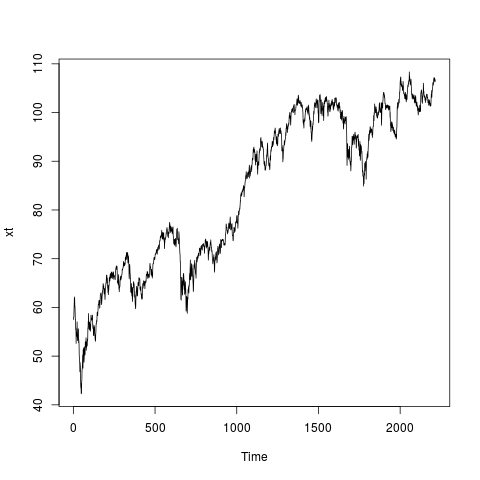
\includegraphics[width=100mm]{/home/taylor/UVa/all_teaching/4170_slides/8/multiv_garch/Rplot.png}
\end{center}

\end{frame}

%----------------------------------------------------------------------------------------

\begin{frame}
\frametitle{Restrictions}

\begin{enumerate}
\item restrict each $\Gamma_i$ to be diagonal...$K(K+1)/2 + q K(K+1)/2$
\item individual ARCH(q) models: $K + qK$
\item BEKK model: $\Sigma_{t|t-1} = C_0^*C_0^{*'} + \Gamma_1^{*'}u_{t-1}u_{t-1}' \Gamma_1^{*} + \cdots + \Gamma_q^{*'}u_{t-q}u_{t-q}' \Gamma_q^{*}$\\...$K(K+1)/2 + q K^2$ parameters
\end{enumerate}
the last one ensures positive-definiteness, too
\end{frame}

%----------------------------------------------------------------------------------------

\begin{frame}
\frametitle{Definition}

Assume that $\Sigma_{t|t-1}^{1/2}$ is symmetric. 
\begin{block}{ Multivariate GARCH(q,m)}
\[
u_t = \Sigma_{t|t-1}^{1/2}\epsilon_t
\]
\[
\operatorname{vech}\left( \Sigma_{t|t-1}^{1/2} \right)= \gamma_0 + \sum_{i=1}^q \Gamma_i \operatorname{vech}(u_{t-i} u_{t-i}') +  \sum_{j=1}^m G_j\operatorname{vech}(\Sigma_{t-i|t-i-1}^{1/2})
\]
\end{block}



\end{frame}

%----------------------------------------------------------------------------------------

\begin{frame}
\frametitle{Definition}

Idea: separate estimation of the correlations and the variances...
\begin{block}{ Dynamic Conditional Correlation model (DCC)}
Let $h_t$ be the vector of conditional variances
\[
\Sigma_{t|t-1} = D_t R_t D_t
\]
where $D_t = \text{diag}(\sqrt{h_{11,t}}, \ldots, \sqrt{h_{KK,t}} )$ is a diagonal matrix, and $R_t$ is a positive-definite correlation matrix. 
\[
h_t = \omega + \sum_{i=1}^p A_i u_{t-i} \odot u_{t-i} + \sum_{j=1}^q B_i h_{t-i}
\]
\[
\mathbf{Q}_t = \bar{\mathbf{Q}} + a(\epsilon_t \epsilon_{t-1}' - \bar{\mathbf{Q}}) + b(\mathbf{Q}_{t-1} - \bar{\mathbf{Q}})
\]
\[
R_t = \text{diag}(\mathbf{Q}_t)^{-1/2}\mathbf{Q}_t\text{diag}(\mathbf{Q}_t)^{-1/2}
\]
with $a+b < 1$.
\end{block}



\end{frame}

%----------------------------------------------------------------------------------------

\begin{frame}
\frametitle{Example}

Say at time $t$ you have $\Sigma_{t+1|t}$ $\mu_{t+1|t}$. Risk and reward of your future return are
\[
\operatorname{Var}(w' r_{t+1} | r_{1:t}) = w'\Sigma_{t+1|t}w
\]
and
\[
E[w'r_{t+1} | r_{1:t}] = w'\mu_{t+1|t}
\]
respectively.

You can use Lagrange multipliers to minimize $w'\Sigma_{t+1|t}w$ subject to $w'\bm{1} = 1$, and it will yield
\[
w_{\text{opt}} = \frac{\Sigma_{t+1|t}^{-1}\bm{1}  }{ \bm{1} '\Sigma_{t+1|t}^{-1}\bm{1}}.
\]

NB: There are a lot of other options (e.g. take into account expected return, disallowing short-selling, investing in risk-free bonds, other-types of constraints, utility functions, taking into account transaction costs, etc. etc.). This is way outside the scope of this class and probably statistics in general...this is just for illustrative purposes.

\end{frame}

%----------------------------------------------------------------------------------------

\begin{frame}[fragile]
\frametitle{Example R code}

\begin{verbatim}
getMinVarPortfolio <- function(sigma){
  n <- nrow(sigma)
  ones <- matrix(rep(1,n), ncol=1)
  denom <- t(ones) %*% solve(sigma) %*% ones
  solve(sigma) %*% ones / denom[1]
}
\end{verbatim}

\end{frame}


\end{document} 